%%%% 
% This is a template for project reports in the subject DAT620 at the
% Department of Electrical Engineering and Computer Science,
% University of Stavanger.
% 
% The template is based on the ACM conference template 
% it was edited by Leander Jehl and Hein Meling
\documentclass[sigconf]{acmart}

%DON'T CHANGE THIS FILE
%This file sets several properties for the ACM template.
%It is not necessary to change this file.


% Copyright
\setcopyright{none}

% DOI
\acmDOI{}

% ISBN
\acmISBN{}

%Conference
\acmConference[Program Analysis for cybersecurity(CP8320)]{}
\acmBooktitle{}
\copyrightyear{2021}

\newcommand{\supervisors}[1]{\thanks{Supervised by #1}}



%In the preamble file you can include packages and define macros.
\usepackage{xspace}

%Here we define a marco: The \xspace ensures correct spacing, i.e. insert space before next word, but not before period or comma.
\newcommand{\paxos}{\textsc{Paxos}\xspace}

%These packages are needed for the plot in Figure 1. 
\usepackage{algorithm}
\usepackage{algpseudocode}
\usepackage{seqsplit}
\usepackage{amsmath}
\newcommand{\urlline}[1]{{\ttfamily\seqsplit{#1}}}
% \pgfplotsset{compat=newest}



\begin{document}
%TODO: Replace the title with your project title.
\title{DeeperXSS: An Exploration of the DeepXSS Approach}
%you may use a subtitle
% \subtitle{My project subtitle}

%TODO replace author names with your name and email below:
\author{Matthew Bush, Dawson Brown}
\affiliation{Ryerson University, Toronto, Canada}
\email{matthew.bush@ryerson.ca, dawson.brown@ryerson.ca}

%TODO: add the name of one or more supervisors
\supervisors{Prof. Manar Alalfi}



\begin{abstract}
%The abstract lies in a different file: 
\textbf{Cross-site scripting (XSS) attacks pose a major threat to the current Web. XSS very regularly ranks among the top ten most common attacks and vulnerabilities on the Web. As such, the successful detection and prevention of such attacks remain an active and important area of research. In this paper, we set out to replicate, critique, and expand on the DeepXSS approach proposed by Fang \text{et al.} This paper gives a lackluster presentation of an LSTM classifier that boats very high precision and recall rates. In order to better understand the application of Deep Learning techniques to XSS classification problems, we dissect their approach, try to recreate their impressive results and contribute some modifications, extensions, and alternative architectures. With this, we hope to justify and critique some of their choices, and provide some context as what works and what doesn't in Deep Learning XSS classifiers.}

\end{abstract}


%TODO: Replace with some keywords, relevant for your project
\keywords{Cross-site Scripting, Deep Learning, LSTM, Word2Vec.}

\maketitle

%Each section can be placed in a separate file and included by the input command.

\section{Introduction}
\label{sec:introduction}
Cross-site scripting (XSS) attacks persist as a major issue for web applications despite their root causes being well understood. XSS is vulnerability by which attackers can inject malicious code into an HTML page which is then recieved and executed by a victims browser. With ever more sensitive data being transacted with on the Web, the personal and industrial consequences of XSS are ever increasing \cite{andreeva2016industrial}. XSS can be split into three broad categories: persistent, reflected, and DOM \cite{gupta2017cross}. Persistent XSS is when an attacker manages to save malicious code on server to be served later to victims; Reflective is occurs when a server echos back a portion of the request--if an attacker can get unsanitized malicious code to be echoed to a victims machine (by having the vitim click a malicious link) the code will be executed in the browser; And lastly DOM is when the attack is executed by modifying the DOM of the victims browser \cite{gupta2017cross}. The Open Web Application Security Project (OWASP) consistently ranks XSS in the top ten vulnerabilities on the Web, including in their most recent 2021 survey (however XSS was lumped into the generic 'injection' category in 2021 instead of having its own category) \cite{owasp}. 

For this reason, there exists a large body of work aimed at automating the detection and prevention of XSS attacks; this includes approaches using Machine Learning techniques to detect both attacks and vulnerabilities. DeepXSS is an LSTM classifier that is meant to detect XSS payloads in reflected XSS attacks; it was designed by Fang \textit{et. al} and is purported to have very high precision and recall rates \cite{fang2018deepxss}. We want to more clearly outline and comment on the strengths and weaknesses of their architecture as well as replicate their purported results.\cite{fang2018deepxss}. 

The primary motivation for this work is to verify Fang \textit{et. al}'s DeepXSS method of detecting cross-site scripting (XSS) attack payloads \cite{fang2018deepxss}. Given the significance of XSS attacks on the Web, there is a need to scrutinize and better understand detection and prevention techniques to better understand what works and what doesn't. We found that DeepXSS lacked detail and failed to address key questions related to their work and so required deeper investigation. Given DeepXSS' promising results, it would be very useful to address the lack of detail, and attempt to replicate the methods used by the authors.  In verifying these results we could further our understanding of why DeepXSS was so effective (or why it was not as effective as it seemed) and apply those lessons to future research. Our main contributions are as follows:

\begin{enumerate}
    \item A custom built URL decoder
    \item An extension of DeepXSS's tokenization technique
    \item A successful recreation of DeepXSS's Word2Vec application
    \item A successful recreation of DeepXSS's LSTM classifier result
    \item Seven additional LSTM models that vary in their input, embedding and/or output to compare and contrast some of the choices made in DeepXSS
\end{enumerate}

The rest of this paper is organized as follows: first we give a brief overview of DeepXSS highlighting its limitations in terms of reproducibility, then we outline our DeeperXSS approach where we recreate (with some modifications) the DeepXSS architecture, then we evaluate our models using 10-fold cross validation, we then go over some related work that factored into our decision making when trying to recreate this work, lastly we give a brief discussion and conclusion.

\section{Background: DeepXSS}
\label{sec:background}
Fang \textit{et al.} claim to make 3 contributions in DeepXSS:

\begin{enumerate}
\item a decoder to undo URL obfuscation
\item a Word2Vec model to embed token strings
\item an LSTM classifier to detect XSS
\end{enumerate}

The decoder is a function that will recursively try to decode `all' possible URL encoding techniques \cite{fang2018deepxss}. Precisely what is meant by `all' encodings is unspecified nor is any source code provided. They however claim to be able to restore arbitrarily obfuscated data \cite{fang2018deepxss}.

After decoding, they `generalize' the resulting URLs. They map all domain names to simply `website', all numbers to `1' and all string parameters to ``param\_string''. They also remove blank and control characters \cite{fang2018deepxss}. They give little justification for this and this step does not seem to affect feature extraction (tokenization) as parameters and numbers aren't tokenized (see table \ref{tok:tab}). 

The tokenization is the first step in feature extraction. They turn each URL into a sequence of tokens according to custom regexes. They do not provide those regexes, they merely provide a table summarizing the types of tokens being extracted (table \ref{tok:tab}) \cite{fang2018deepxss}. The tokens chosen appear to target only the types of strings that would be present in XSS payloads and many benign URLs contain no tokens. It appears that the classifier doesn't come to learn what benign URLs look like as the vast majority contain no features. 

\begin{table}
\begin{center}
\begingroup
\setlength{\tabcolsep}{5pt} % Default value: 6pt
\renewcommand{\arraystretch}{1.5} % Default value: 1
\begin{tabular}{||c | c||} 
    \hline
    Classification & Example \\ [0.5ex] 
    \hline\hline
    \textbf{Start Label} &  $<$script$>$, $<$body$>$, $<$img \\ 
    \hline
    \textbf{End Label} & $</$script$>$, $</$body$>$ \\
    \hline
    \textbf{Windows Event} & onerror=, onload=, onblur=, oncut= \\
    \hline
    \textbf{Function Name} & alert(, String.fromCharCode( \\
    \hline
    \textbf{Script URL} & javascript:, vbscript: \\ 
    \hline
    \textbf{Other} & $>$, ), \# \\ [1ex] 
    \hline
\end{tabular}
\endgroup
\caption{\label{tok:tab}DeepXSS Tokens.}
\end{center}
\end{table}

Once the URLs have been tokenized, they use the continuous bag of words (CBOW) model to perform word embedding on the token strings \cite{fang2018deepxss}. They do this to extract the semantics of the tokens and provide more features to the LSTM classifier \cite{fang2018deepxss}. They do not specify the numbder of dimensions their word vectors have nor the number of epochs used while training the CBOW model; CBOW is, of course, sensitive to both \cite{mikolov2013efficient}.

Once the word vectors are trained, the LSTM can be trained by feeding it sequences of word vectors representing URLs \cite{fang2018deepxss}. 

\section{Our Approach: DeeperXSS}
\label{sec:method}
In this section we outline our approach for recreating the DeepXSS architecture, including difficulties we had in reproducibility, limitations with DeepXSS that needed to be addressed, some creative liberties we took, and a few alternative machine learning architectures that proved interesting. 

\subsection{Data Preprocessing}
\subsubsection{Decoding}
We built a custom recursive URL decoder. This decoder performs a depth first search of 5 different decodings. At each level, the decoder tries to decode the URL with all decodings, for each decoding that is successfull, the decoder will recursively try to further decode the string that resulted from the decoding; see algorithm \ref{decoder} for a pseudocode implementation. The first string enoucountered that none of the decoders can decode is returned as the decoded string. The supported encodings are: URL unicode encoding (this includes characters of the form \%uxxxx and \textbackslash uxxxx),URL encoding (that is characters of the form \%xx), HTML character references (that is characters of the form \&xx;), hex encoding, and base64 encoding. 

Algorithm \ref{decoder} works as follows: on line \ref{dec:all} all the decoder functions are called and passed the URL to be decoded. These functions all return a Tuple of the form (Boolean, String) where the Boolean value indicates if the decoding was successfull while the String is the decoded string (the String remains unchanged if the decoding fails). Next, on line \ref{dec:res}, the result tuples of all the attempted decoders are looped over. If it's found that a decoder was successful (line \ref{dec:check}) then recurisvely call the decoder on the resulting string (line \ref{dec:rec}). If the recursive decoding succeeds than return the result of the recursive call (\ref{dec:rec:true}). If the decoder gets to line \ref{dec:nrec}, than that means one of two things happened: either none of the decoders succeeded, in which case the string must be fully decoded and so we go to line \ref{dec:true}; if on the other hand some of the decoders succeeded, then if the algorithm gets to line \ref{dec:nrec} it must have been the case that none of the recursive calls succeeded (meaning line \ref{dec:rec:true} was never reached) which means the decoder was unable to decode the string and we return on line \ref{dec:false}. 

\begin{algorithm}
\caption{Recursive Decoder}\
\label{decoder}
\begin{algorithmic}[1]
    \Function{decode}{url}
        \State decoders $\gets$ [url(), unicode(), html(), hex(), base64()]
        \State dec\_results $\gets$ []
        \For{decoder \textbf{in} decoders} \label{dec:all}
            \State dec\_results.append(decoder(url))
        \EndFor

        \State some\_decoded $\gets False$
        \For{decode\_success, decode\_str \textbf{in} dec\_results} \label{dec:res}
            \State some\_decoded $\gets$ decode\_success \textbf{or} some\_decoded
            \If{decode\_success} \label{dec:check}
                \State (next\_decode\_success, next\_decode\_str) = DECODE(decode\_str) \label{dec:rec}
                \If{next\_decode\_success}
                    \State \Return ($True$, next\_decode\_str) \label{dec:rec:true}
                \EndIf
            \EndIf 
        \EndFor

        \If{some\_decoded} \label{dec:nrec}
            \State \Return ($False$, url) \label{dec:false}
        \Else 
            \State \Return ($True$, url) \label{dec:true}
        \EndIf

    \EndFunction
\end{algorithmic}
\end{algorithm}

To clarify with an example, consider the URL:

\urlline{http://example.com/706174682F746F2F66696C653F783D26616D703B6C743B73637269707426616D703B67743B253230616C65727428253230312532302925323026616D703B6C743B2F73637269707426616D703B67743B}. 

Passing this through the decoder, the Hex decoder will succeed and produce the string: 

\urlline{http://example.com/path/to/file?x=\&amp;lt;script\&amp;gt;\%20alert(\%201\%20)\%20\&amp;lt;/script\&amp;gt;} 

then the URL decoder will succeed giving the string: 

\urlline{http://example.com/path/to/file?x=\&amp;lt;script\&amp;gt; alert( 1 ) \&amp;lt;/script\&amp;gt;}

then the HTML decoder will succeed and give:

\urlline{http://example.com/path/to/file?x=\&lt;script\&gt; alert( 1 ) \&lt;/script\&gt;} 

and finally the HTML decoder will succeed again and give: 

\urlline{http://example.com/path/to/file?x=<script> alert( 1 ) </script>}. 

No decoders will succeed here making this the final form.


\subsubsection{Tokenization}
As seen in table \ref{tok:tab}, DeepXSS defined six different token types. We expanded on this set of tokens and ended up with a total of 14 token types. The reason we expanded on this token set is because many URLs contained zero tokens. For example \url{http://www.wittebeer.be/?oid=911\&pid=8056} or \url{http://www.facebook.com/Euphnet?sk=wall}, both of which are in the DMOZ directory, do not contain any of their token types. Using more token types common to normal URLs and increasing the feature richness as a way to have benign samples not be empty was something we encountered in the literature \cite{mokbal2019mlpxss}\cite{zhang2019cross}. But put basically, we didn't want our classifier to come to learn that benign URLs are largely empty; we wanted it to learn the structure of both benign and malicious URLs. As such, we expanded their table to include 8 more as shown in table \ref{exp:tok:tab}.


\begin{table}
\begin{center}
\begingroup
\setlength{\tabcolsep}{5pt} % Default value: 6pt
\renewcommand{\arraystretch}{1.5} % Default value: 1
\begin{tabular}{||c | c||} 
    \hline
    Classification & Example \\ [0.5ex] 
    \hline\hline
    \textbf{Integer Argument} &  (543), (1), (2004) \\ 
    \hline
    \textbf{Integer Constant} &  1, 2, 5432, 54 \\ 
    \hline
    \textbf{String Argument} & (``Hello''), (String.fromCharCode(65)) \\
    \hline
    \textbf{Assignment LHS} & x=, variable= \\
    \hline
    \textbf{Assignment RHS} & =x, =654, =value \\
    \hline
    \textbf{Path} & path/ t56543-trer-yt43/ \\ 
    \hline
    \textbf{Identifier} & iden, value, hello, goodbye \\ [1ex] 
    \hline
\end{tabular}
\endgroup
\caption{\label{exp:tok:tab}Extended DeepXSS Tokens.}
\end{center}
\end{table}

An integer argument token is any integer value that follows a function name token and is enclosed in brackets. Similarly, a string argument token is taken to be any argument that isn't an integer; hence \textit{String.fromCharCode(65)} being an example of a string argument. We figured that distinguishing futher between arguments would be superfluous, and by inspection these were the most common arguments (including functions which returned a string or integer). The integer constant token was introduced because many URLs contained non-descript integers outside of function calls and URL arguments. The two assignment tokens (left-hand side and right-hand side) were introduced so that URL arguments would not be lost (notice that the two benign examples include arguments that are skipped by DeepXSS). Similarly, path tokens were intoduced so that the path wasn't entirely skipped. And finally we introduced a generic identifier token. Assignment LHS, Path, Script URL, Function Name, and Windows Events all begin with an identifier but all have additional characters to further distinguish them (for example Windows Events always start with `on' and end with `=', paths end with `/' or `?', etc). Any identifier that is found that cannot be further categorized is included as a generic Identifier token.

\subsubsection{Generalization}
In keeping with DeepXSS, we generalized many parts of the URL. In the original paper all the domains became simply `website'. Having every URL begin with `http://website' communicates no information and so we simply ommitted the domain. We mapped all integer arguments to `(1)' and all string arguments to `(``str\_arg'')'. All integer constants were mapped to `1'. The left-hand side of assignments were all generalized to `assign<num>=' where `<num>' starts from 0 and increments for each encountered left-hand side. This was done because most identifiers in URLs proved to be unique, and so not useful in classification (especially when using CBOW) with the exception of Function Names, script URLs, and Windows Events which are reserved words and so can't be unique across many URLs. The right-hand sides are generalized to `val<num>' where `<num>' again increments with each right-hand side encountered. Similarly, all path tokens are generalized to `path<num>/' and finally all identifier tokens were mapped to `ident<num>'.

To clarify the tokenization and generalization process with an example, consider \urlline{http://website/search.php?uid=ws848d8024088c327.36898031\&src=\&term=<script>alert(123)</script>\&args=qs=06o}. The following sequence of (token type, token value) pairs would be extracted going left to right:


\begin{lstlisting}[caption=Example tokenization, label=tokenization]
(Path, `path0/') for search.php?
(Assignment LHS, `assign0=') for uid=
(Assignment RHS, `val0') for =ws848d8024088c327
(Integer Constant, 1) for 36898031
(Assignment LHS, `assign1=') for src=
(Assignment LHS, `assign2=') for term=
(Start Label, `<script>') for <script>
(Function Name, `alert') for alert(
(Integer Argument, `(1)') for (123)
(End Label, `</script>') for <script>
(Assignment LHS, `assign3=') for args=
(Assignment LHS, `assign4=') for qs=
(Integer Constant, `06') for 06
(Identifier, `o') for o
\end{lstlisting}


Note that if two different token types overlap, the one that starts earlier is preferred; if they start in the same place then the one that extends further is preferred. This is why `args=qs=' is taken to be two left-hand sides--the `qs' could be a right-hand side, but with the equals on the right its taken to be a left-hand side since that is longer and both start at the `q'. As per the last two tokens, identifiers cannot start with numbers  (in Javascript) and so the 06o is taken to be an integer constant followed by an identifier.


\subsection{Word2Vec}

As one of the primary stated contributions of the original DeepXSS \cite{fang2018deepxss} paper, properly implementing CBOW for Word2Vec is an important part of our recreation. Unfortunately, the authors do not give good indication as to how CBOW was applied, merely stating that CBOW was used to construct word representations. We therefore took liberties with our implementation and based many decisions on the work from \cite{afzal2021deeplearning}. One major point of confusion was whether CBOW representations were constructed for token type labels, or the token itself. To test the difference, we implemented both.

In order to generate the CBOW embeddings we first needed to build a vocabulary of tokens with each token represented by a unique integer. Zeros represent padding tokens which are used later in the process.  Once the vocabulary is constructed, each list of URL tokens is replaced with corresponding integer representations.  Every vectorized URL is then padded with zeros until they are all a uniform length.  The padding tokens ensure that empty space does not influence the outcomes of the model.
Figure \ref{cbow-arch} shows the architecture for the model we use to generate our CBOW embeddings.  For every token in our vectorized URL, the CBOW model attempts to predict the current token using the tokens around it.  Using a window size of two means that our CBOW model will attempt to predict the middle token using two adjacent tokens on either side of it.  As the model does this for every token in the dataset, the weights of the embedding layer are trained.  The embedding layer is responsible for taking each token and turning it into a multidimensional representation.  In the case of token type labels, each token will have a ten-dimensional representation and token values receive a 50-dimensional representation.

\begin{figure}[H]
    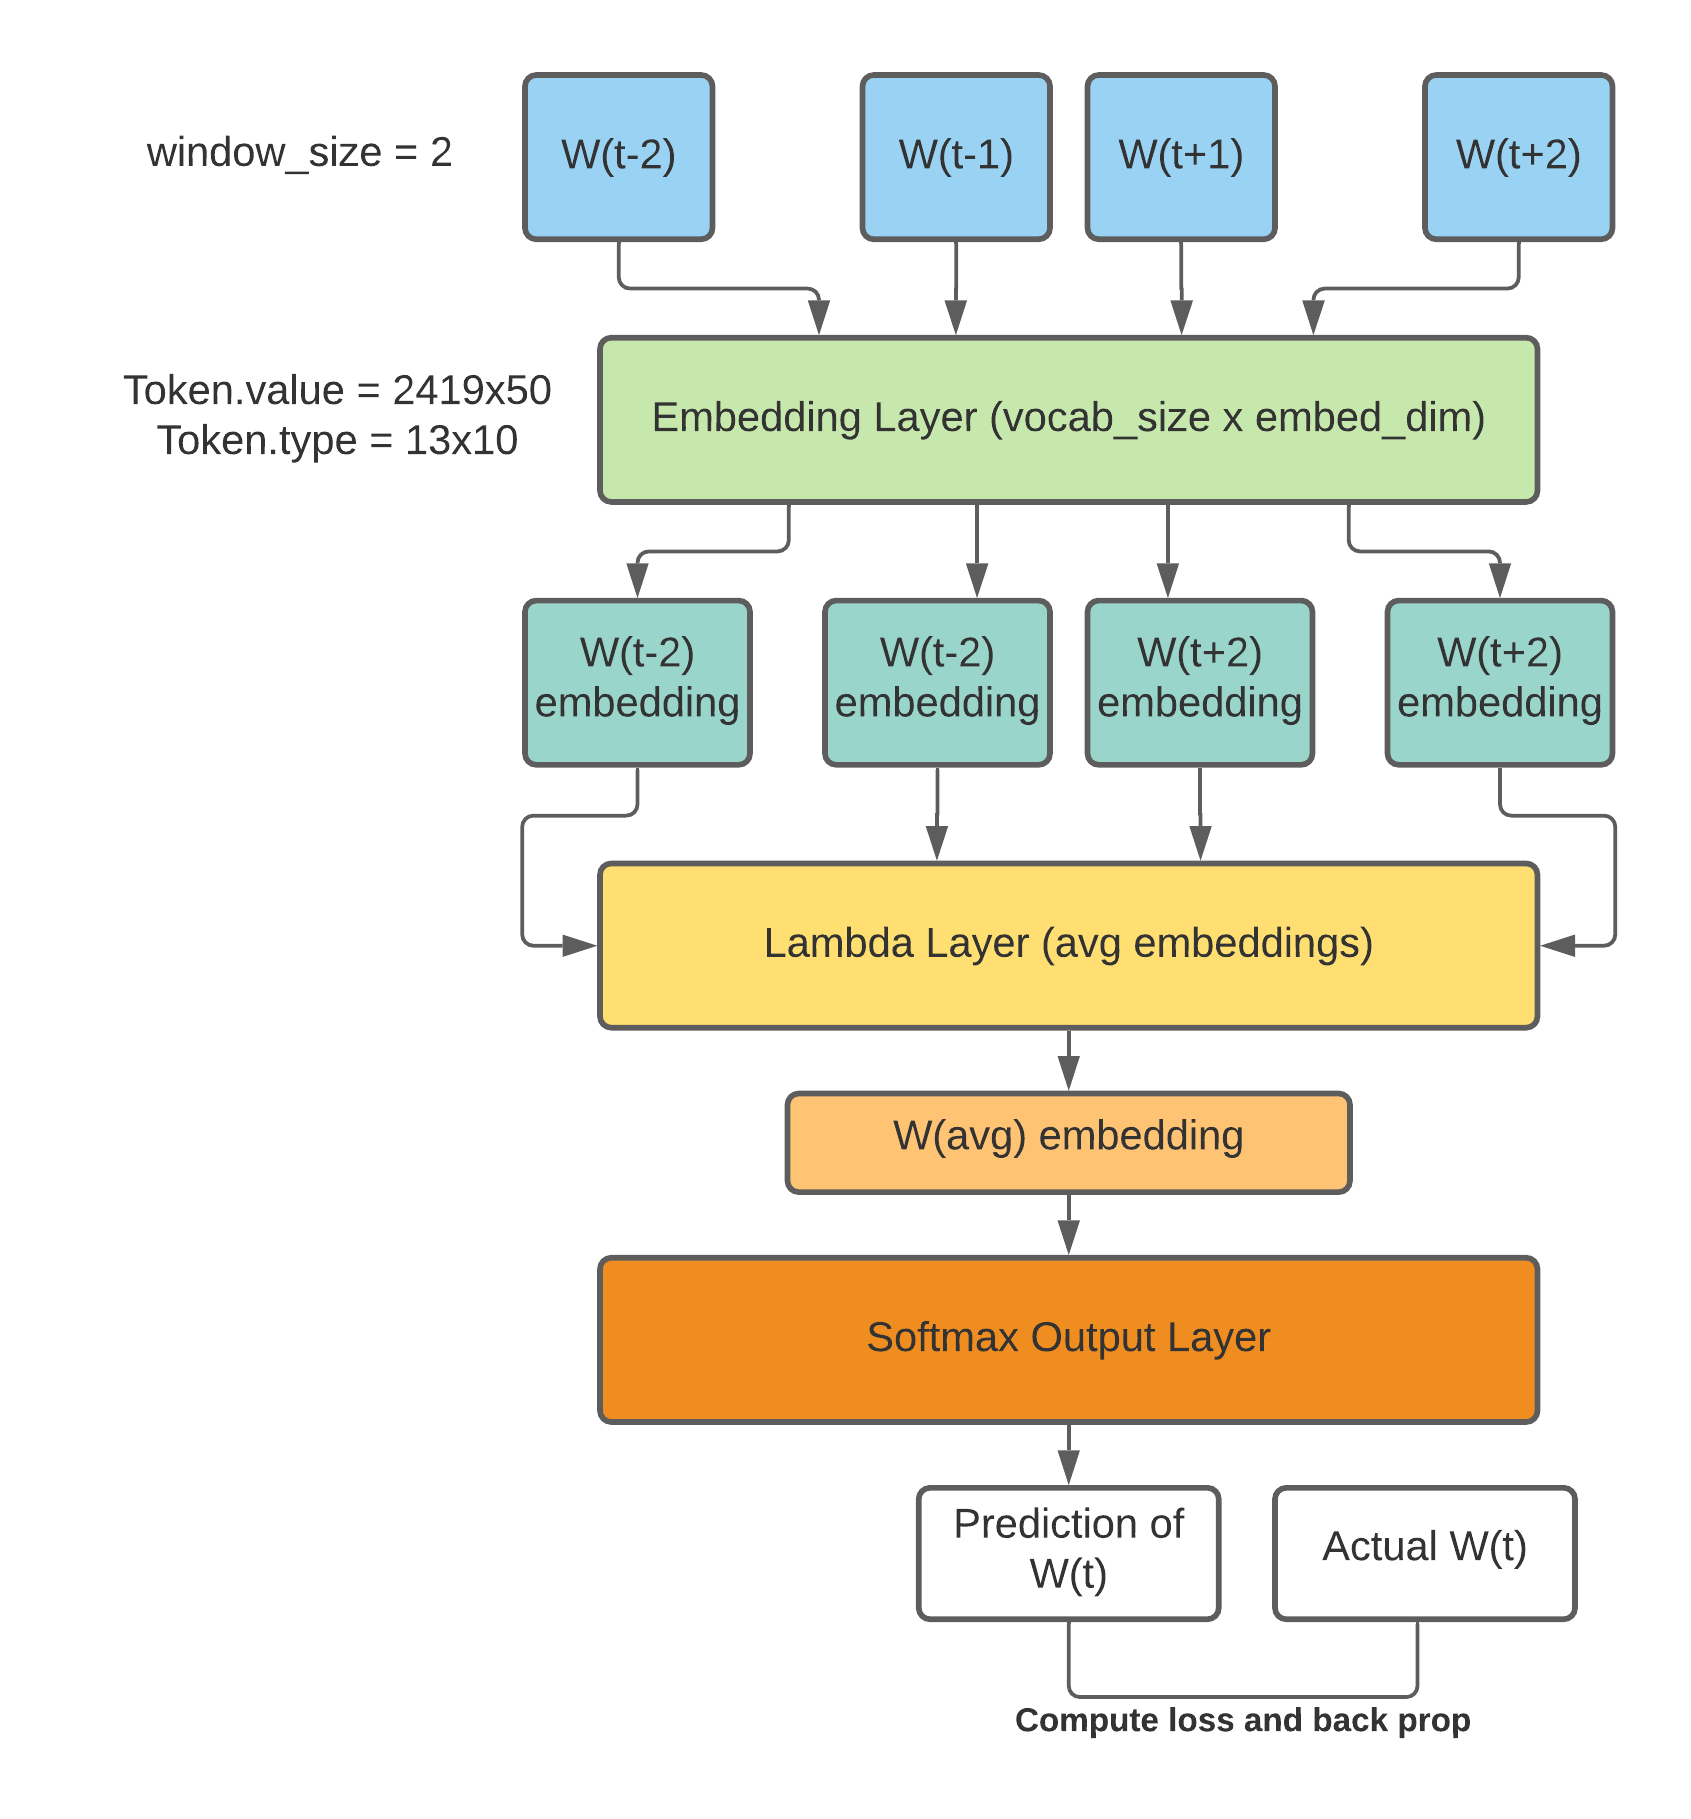
\includegraphics[width=0.45\textwidth, angle=0]{cbow_model}
\end{figure} \label{cbow-arch}

\begin{lstlisting}[caption=Related token values, label=cbow-exp-value]
<script>: >,ident1,</title>,path4/,<h1>
alert: ident11,ident13,ident12,<img>,path4/
</script>: <h1>,<marquee>,ident2,ident4,ident5
(1): ident4,<"<<script>,javascript,</style>,</title>
path0/: assign0=,ident1,ident0,</title>,<iframe>  
\end{lstlisting}



\begin{lstlisting}[caption=Related token types, label=cbow-exp-type]
path: int_const,value,int_arg,func_name,assign
int_const: path,value,assign,func_name,int_arg
assign: value,other,int_cons,int_arg,str_arg
value: assign,other,int_const,int_arg,func_name
ident: other,start_label,value,assign,int_arg  
\end{lstlisting}

Extracting the weights from the embedding layer and calculating the Euclidean distance between tokens allows us to see an example of similar words according to our CBOW embeddings. Listing \ref{cbow-exp-value} shows examples of the five most closely related token values and Listing \ref{cbow-exp-type} shows examples of the five most closely related token types.

Training each new CBOW model on the entire dataset could take as many as 24 hours meaning we needed to make changes to the tokenization process to produce better generalized data.  This sped up CBOW generation but likely resulted in some lost semantic information.


\subsection{LSTM Classifier}

The final stated contribution of DeepXSS \cite{fang2018deepxss} and arguably the most important is the LSTM classifier for XSS detection.  The authors provide a brief description of this classifier stating that it has three layers: an LSTM layer, a dropout layer to reduce overfitting, and a softmax output layer that makes predictions.  We had two primary difficulties in reconstructing the model from this description.

The first difficulty was with using the embedded token vectors in the LSTM.  We often had large numbers of embedded token vectors for every URL.  This resulted in large, nested arrays of data that were difficult to work with. We chose to transplant a non-trainable embedding layer from our CBOW model into the LSTM model as shown in \ref{lstm_model}.  This allows us to simply feed the model sequences of integers where the embeddings are constructed within the model rather than during preprocessing.

\begin{figure}[H]
	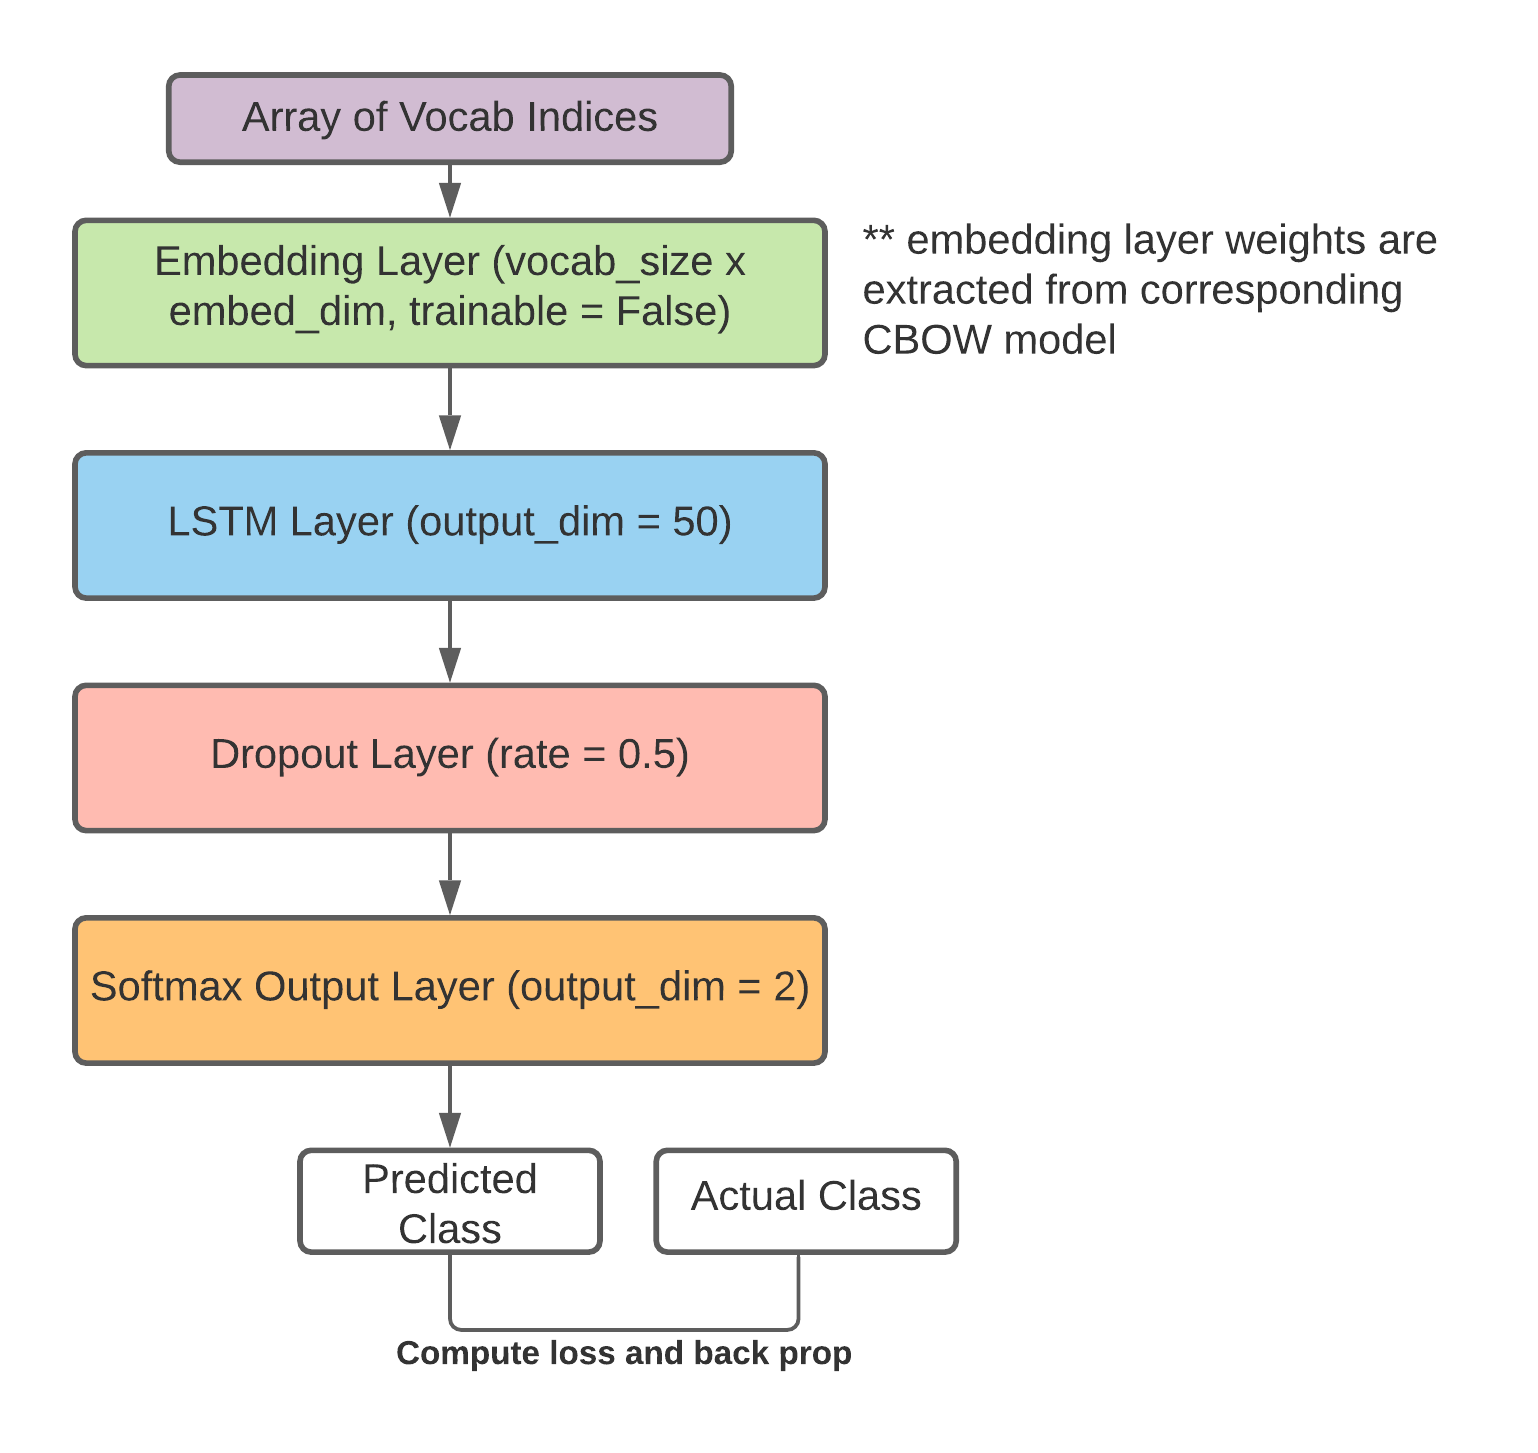
\includegraphics[width=0.8\textwidth, angle=0]{lstm_model}
\end{figure}

The other difficulty we had with constructing and training the LSTM model was with hyperparameters and model details. We found that the LSTM was often very difficult to train, seemingly making no progress after multiple epochs.  Experimenting with dropout rates, the output size of the LSTM, and several other factors was extremely time consuming.  Eventually we were able to settle on the model in \ref{lstm_model} as our primary architecture for both token type and token value.

We also constructed other models to test the importance of various design choices from the original DeepXSS paper \cite{fang2018deepxss}.  The first model is our primary design that is shown in \ref{lstm_model}. We also created a model with a sigmoid output layer, given that a softmax output layer is somewhat unnecessary for a dual classification model.  Another model is intended to test the value of the CBOW embeddings by simply training the model on sequences of integers that map to all of the tokens.  This model has no embedding layer.  The final model has an untrained embedding layer to test if the CBOW embeddings needed to be trained separately or if word embeddings could be learned through normal training.  All of these models exist for both token type and token value resulting in eight models total.  The models are listed in \ref{model-sum}.



\begin{table}
\begin{center}
\begingroup
\setlength{\tabcolsep}{6pt} % Default value: 6pt
\renewcommand{\arraystretch}{1.5} % Default value: 1
\begin{tabular}{|| c | c | c | c ||} 
    \hline
    Model & Output & Embedding & Input \\ 
    \hline\hline
    \textbf{Value-Softmax} & softmax & CBOW & Token values \\
    \hline
    \textbf{Value-Sigmoid} &  sigmoid & CBOW & Token values \\ 
    \hline
    \textbf{Value-Sequential} & softmax & None & Token values \\
    \hline
    \textbf{Value-Random} & softmax & Random & Token values \\
    \hline
    \textbf{Type-Softmax} & softmax & CBOW & Token types \\
    \hline
    \textbf{Type-Sigmoid} & sigmoid & CBOW & Token types \\
    \hline
    \textbf{Type-Sequential} & softmax & None & Token types \\
    \hline
    \textbf{Type-Random} & softmax & Random & Token types \\
    \hline
\end{tabular}
\endgroup
\caption{\label{model-sum}Summary of Models}
\end{center}
\end{table}


\section{Evaluation}
\label{sec:evaluation}
\begin{table}
\begin{center}
\begingroup
\setlength{\tabcolsep}{10pt} % Default value: 6pt
\renewcommand{\arraystretch}{1.5} % Default value: 1
\begin{tabular}{|| c | c | c ||} 
    \hline
    Prediction & XSS & Not XSS \\ 
    \hline\hline
    \textbf{Predicted XSS} &  $t_p$ & $f_p$ \\ 
    \hline
    \textbf{Predicted Not XSS} & $f_n$ & $t_n$ \\
    \hline
\end{tabular}
\endgroup
\caption{\label{conf-mat}Confusion Matrix}
\end{center}
\end{table}


\begin{align*}
    &\text{Precision} = \frac{t_p}{t_p + f_p} \\[10pt]
    &\text{Recall} = \frac{t_p}{t_p + f_n} \\[10pt]
    &\text{F1} = 2 \cdot \frac{\text{Precision} \cdot \text{Recall}}{\text{Precision} + \text{Recall}}\\[10pt]
    &\text{Accuracy} = \frac{t_p + t_n}{t_p + t_n + f_p + f_n}
\end{align*}

\begin{table}
\begin{center}
\begingroup
\setlength{\tabcolsep}{4pt} % Default value: 6pt
\renewcommand{\arraystretch}{1.5} % Default value: 1
\begin{tabular}{|| c | c | c | c | c ||} 
    \hline
    Model & Precision & Recall & F1 & Accuracy \\ 
    \hline\hline
    \textbf{DeepXSS} &  0.995 & 0.979 & 0.987 & n/a \\ 
    \hline
    \textbf{DeeperXSS:softmax} & 0.989 & 0.973 & 0.981 & 0.981 \\
    \hline
    \textbf{DeeperXSS:sigmoid} & 0.988 & 0.976 & 0.982 & 0.983 \\
    \hline
    \textbf{DeeperXSS:sequence} & 0.991 & 0.956 & 0.973 & 0.975 \\
    \hline
    \textbf{DeeperXSS:random} & 0.099 & 0.097 & 0.098 & 0.56 \\
    \hline
\end{tabular}
\endgroup
\caption{\label{comparison}Model Comparison.}
\end{center}
\end{table}

\section{Related Work}
\label{sec:related}
Mokbal \textit{et al.} created a multilayer perceptron (MLP) model for detecting XSS both in dynamic webpages and URLs \cite{mokbal2019mlpxss}. Their approach, called MLPXSS, has three main pillars: data scraping, feature extraction, and an artificial neural network (ANN). Their feature extraction level has three modules to extract HTML-based features, Javascript-based features, and URL-based features. The HTML module tokenizes tags, attributes and events--focusing on things that trigger Javascript execution (like \textit{href} or \textit{onclick}). The Javascript module parses and tokenizes Javascript code that is pulled from a webpage creating an abstract syntax tree. There are various ways to include Javascript in a page like script tags, \textit{onclick} and \textit{onsubmit} calls, \textit{href}, etc... Lastly they tokenize potentially malicious parts of URLs, like HTML properties, tags, some keywords (\textit{login}, \textit{signup}), \textit{document} references, and various special characters like `$<$', `$>$' and `$/$'. The MLP is trained on token streams with a sigmoid output layer. Their perceptron had precision, f-measure, and accuracy all in excess of 99\% \cite{mokbal2019mlpxss}.

Zhang \textit{et al.} propose a dual Gaussian mixture model (GMM) approach that trains two seperate GMMs models (one for benign and one for malicious) and then combines their outputs to make a prediction. Additionally, they train the models on both the URL and the server response to the URL in an attempt to get richer features \cite{zhang2019cross}. To preprocess the URLs, they decode, tokenize, and train a Word2Vec model to retrieve a vector representation of each token. Their tokenization approach is very similar to that of DeepXSS and MPLXSS, they however inclue the domain and path for the benign GMM. They are however generalized to simply `domain' and `path' \cite{zhang2019cross}. Their reasoning for this is that containing just a domain and path is characteristic of a benign URL, whereas an XSS URL is characterized by its maliciously constructed parameters and not the presence of a domain and path \cite{zhang2019cross}. Their models can be trained on requests, responses, or both. They reason that in many cases, benign requests contain no XSS tokens, which isn't very interesting, however responses contain useful features for both XSS and none-XSS tokenization. Their multi-stage dual GMM using both responses and requests greatly improved classification \cite{zhang2019cross}.

Goswami \textit{et al.} propose an attribute clustering technique to perform unsupervised grouping of malicious and benign scripts. They're feature extraction is wholly different from DeepXSS and other deep learning classifiers. They propose 15 features that characterize malicious and benign scripts creating a 16-dimensional vector for each script (including class) \cite{goswami2017unsupervised}. These features are meta-features like length of the script, number of strings and the average string length, number of methods, number of unicode and hex characters, among others. These features are then min-max normalized before clustering \cite{goswami2017unsupervised}. Their algorithm was able to achieve an accuracy in excess of 98\% \cite{goswami2017unsupervised}.  

The authors in \cite{afzal2021deeplearning} focus on classifying broadly defined malicious URLs sent through email or over social networks.  In this case a malicious URL is any URL that could result in harm to the user visiting it.  They propose a hybrid deep-learning approach called \textit{URLdeepDetect} to extract semantic features from URLs to classify them as either benign or malicious.  The preprocessing stages tokenizes various parts of the URL before applying word-level embedding through Word2Vec.  The embedded tokens are then fed to an LSTM where samples are classified based on LSTM outputs or k-means clustering.  This paper claims 98.3\% accuracy for LSTM classification of malicious URLs and 99.7\% accuracy with k-means clustering.  The authors claim that the success of their approach is in part due to the Word2Vec token embedding and maintaining URL sequence as it provides the model with more semantic information for classification.

The work done in \cite{vishnu2014prediction} explores XSS detection using three machine learning algorithms: Naïve Bayes, Support Vector Machine, and J48 Decision Tree.  This paper attempts to detect reflected XSS, persistent XSS, and DOM based XSS meaning it requires web page scripts as well as URLs.  The malicious URLs and scripts were collected from the XXSed \cite{xssed} project and the benign samples were collected from the Dmoz open directory project \cite{dmoz}.  This work, however, only uses five features for scripts (e.g., number of characters, request for cookie, etc.) and seven features for URLs (e.g., number of characters, presence of script tags, etc.) rather than extracting tokens to represent the entire URL or script.  Each model was then subjected to 10-fold cross validation and the results were compared.  J48 performed the best based on features from both URL and JavaScript achieving a 99\% true positive rate and 99\% precision.  The authors also found that discretized attributes provided the best classifier results for J48.

Detecting XSS attacks on social networking sites is the primary focus of \cite{rathore2017xss}.  The authors propose an approach consisting of feature identification, web page collection, feature extraction, building a training dataset, and using a machine learning algorithm to classify web pages as XSS or non-XSS.  This approach extracts features from URLs, HTML tags, and the host social networking site.  The features of these web pages are very coarse-grained, consisting of things like the maximum size of URLs, and counts of harmful keywords.  The authors then train ten classifiers with a RandomForest classifier achieving 97.7\% precision and 97.1\% recall.  They suggest future work to enhance the feature set and apply more machine learning algorithms such as deep learning.

\section{Discussion}
\label{sec:discussion}
This approach is entirely dependent on the scope and correctness of the decoder. The filter evasion techniques used for XSS can be extremely complicated and can include multiple and mixed encodings with near arbitrary white space \cite{xsscheat}. To demonstrate this sensitivity, we applied the standard blacklist/whitelist sanitizer \textbf{bleach} to both the decoded and non-decoded malicious URLs to test the relative efficacies \cite{bleach}. On non-decoded data, the sanitizer only cleaned 62\% of malicious samples, while on the decoded data it cleaned 91\% of samples, clearly showing the importance of decoding. Furthermore, new evasion techniques are continually being discovered as well. The decoder has to be sophisticated enough to handle the evasion techniques of novel XSS payloads to be useful in practice. That said, a good decoder will be hard to evade and probably only a negligible number of XSS payloads will get past it, on the other hand, given the severity of the consequences of some XSS attacks, no number is negligible. 

As with all machine learning, this approach is very sensitive to the preprocessing of the data and the feature extraction. In our case, this is the tokenization step. There have been many different tokenization procedures proposed; often they exclusively looked for tokens that would indicate a malicious URL and largely ignored the benign segments of a URL \cite{fang2018deepxss}\cite{mokbal2019mlpxss}. This approach means that many benign URLs contain no tokens \cite{zhang2019cross}. This sort of approach requires the designer of the tokens to judge what kinds of strings characterize malicious URLs and only tokenize those which can be hard to do well. To address this, perhaps both the URL and the server's response to it can be tokenized which gives a much richer set of features and would help fill out the empty URLs \cite{zhang2019cross}. This has the drawback of having to interact with the server for each URL which adds overhead--ideally the URL provides sufficient information. In our approach, we had a more general tokenization approach that aimed at tokenizing URLs and not just malicious URLs. The idea being that the machine learning algorithm can be left to figure out what sort of strings and patterns characterize malicious URLs without much input from us. This means benign URLs aren't empty and the server response is not required. That said, there are likely benefits to including special strings that give a strong indication of an XSS payload. 

With regards to the models themselves, our results indicate that we have achieved a successful recreation of the original DeepXSS paper validating claims of highly effective XSS classification \cite{fang2018deepxss}. This is a reasonable conclusion given the empirical effectiveness of deep learning methods for classification problems. DeepXSS does have slightly higher metrics than DeeperXSS and the discrepancies can likely be explained by a few key limitations. We were unable to use the exact dataset used for DeepXSS, we lacked specific details about the Word2Vec implementation and the exact nature of the tokens it was applied to, and we lacked details as to how the embedded tokens were used as inputs to the model. With more time we likely could have improved our results with more training epochs, tuning hyperparameters like the dropout rate, and more rigorous data preparation to remove unsuitable samples.

Interestingly, the results trained with token type and token value are almost identical. The models without token embeddings also perform comparably well to the original.  This calls into question the significance of the Word2Vec step that is cited as a primary contribution of the original work. At best the word embeddings provide a marginal boost to the model’s metrics. One explanation could be that the model does not heavily rely on semantic information surrounding the tokens but rather focuses on features like the presence of specific tokens, the length of the URL, and the sequence particular tokens occur in. This said, a properly trained CBOW embedding layer massively outperformed a randomly initialized embedding layer trained alongside the classifier. Training the CBOW model was necessary in order to produce usable word embeddings. Future work should focus on isolating the most important features for classification.

\section{Conclusion}
\label {sec:conclusion}
Detecting and preventing XSS attacks remains an important domain of research. As such it is all the more important that research into this area remains reproducible and usable for practical purposes. In this paper we recreate, validate the DeepXSS approach for XSS detection. We also make comparisons to additional models to validate various claims. Ultimately we found that while DeepXSS is an extremely effective XSS classifier, claims surrounding the importance of Word2Vec for extracting semantic information are exaggerated. Our results indicate that deep learning should continue to be pursued as a means of classifying XSS. Future work should focus on extending this approach to web pages and embedded scripts to detect stored XSS attacks.  Additionally, expanding the recursive decoder to handle more encodings, and isolating the most important features for detecting XSS is an important extension of this work. The final goal should be integrating these classifiers with working systems so that they can help with real time detection and prevention of XSS attacks.

\bibliographystyle{ACM-Reference-Format}
\bibliography{ref}

\end{document}
